\chapter{Use case: GSI Bot}
\label{chap:usecasegsi}

\begin{chapterintro}

In this chapter, we will describe the prototype we developed for a bot for the GSI web page following the architecture described in chapter \ref{chap:architecture}. We will start with the process to recover the data as Linked Data, to them describe the interface and the modules of the system.
 
\end{chapterintro}

\cleardoublepage

\section{Overview of the system}

Along with the prototype described in chapter \ref{chap:usecasejava}, we have also developed a system with the data from the GSI webpage, including data from the projects, publications and staff. For this, we have similar modules:

\begin{enumerate}
 \item A Javascript client acting as the user interface.
 \item A Python controller, handling the flow of the information in the system
 \item A different ChatScript bot, handling the conversation.
 \item An Apache Solr core, with all the data.
\end{enumerate}

In this case, the data was recovered using a mix of techniques, and integrated into a single core in Solr.

\section{Recovering and storing the data}

Similarly to the previous chapter, the data for this prototype has been recovered and converted into RDF and json formats, 

\subsection{Webpage categories}

We considered three types of data from the GSI web page: the information about the members of the groups, their publications and the projects the groups has taken part of. Each type comes from a different part of the website, and therefore will be considered independently. 

\subsubsection{Projects}

For the projects information, the data is available in different formats in the webpage itself, including RDF/XML, as shown in figure \ref{fig:gsiprojects}

\begin{figure}[!htbp]
    \centering
    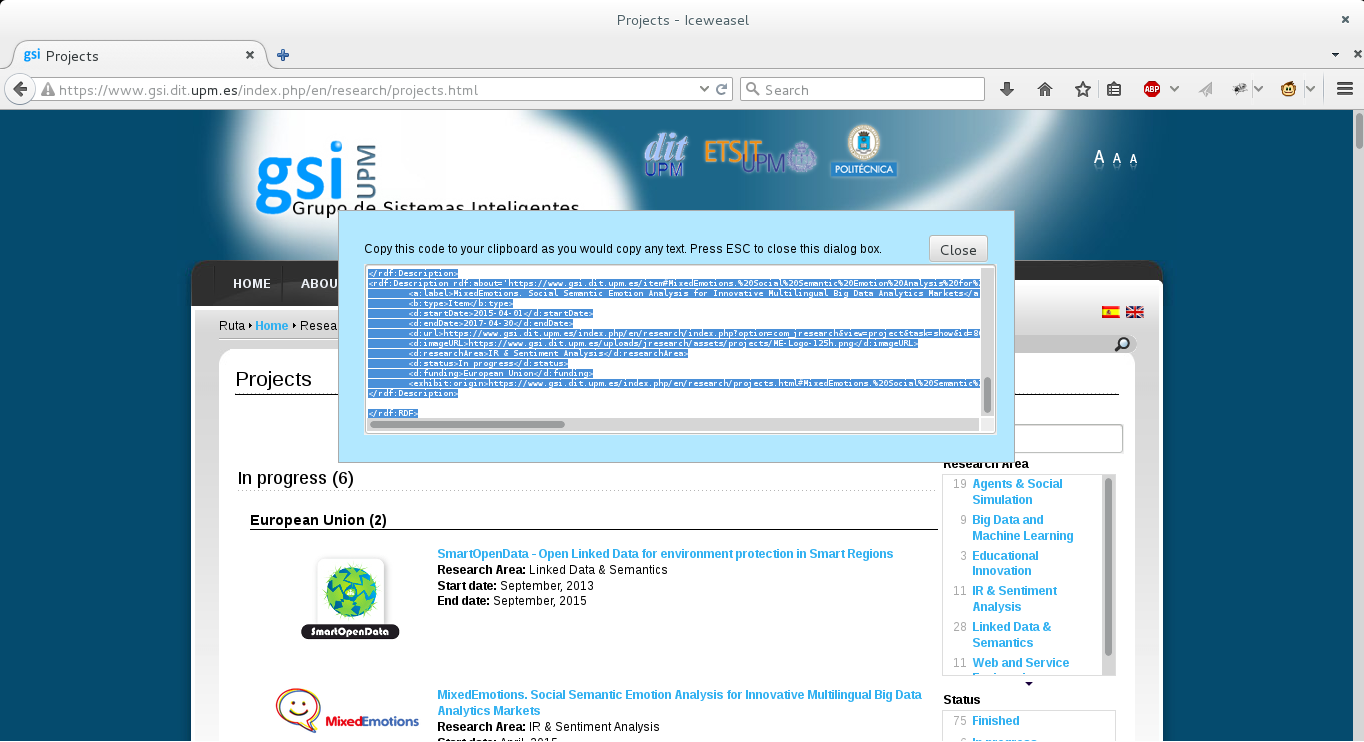
\includegraphics[width=0.8\textwidth]{img/screens/gsi-projects.png}
    \caption{RDF exporter for the projects.}
    \label{fig:gsiprojects}
\end{figure}


\subsubsection{Publications}
\label{subsec:bibtexrdf}

Each publication listed in the GSI webpage has an attached bibtex citation. Therefore, it is possible to use a bibtex ontology\footnote{\url{http://purl.oclc.org/NET/nknouf/ns/bibtex}} to map the elements in the bibtex files to semantic data. The mapping for the classes is shown in table \ref{tab:bibtex-classes}.

\begin{center}
  \begin{table}
    \begin{tabular*}{0.7\textwidth}{@{\extracolsep{\fill}} | c | c | p{0.5\textwidth} |}
      \hhline{|-|-|-|}
      \textbf{Bibtex tag} & \textbf{Ontolgoy mapping} & \textbf{Description} \\ \hhline{|=|=|=|}
      article & bibtex:Article & An article from a journal or magazine. \\ \hhline{|-|-|-|}
      book & bibtex:Book & A book with an explicit publisher. \\ \hhline{|-|-|-|}
      conference & bibtex:Conference & An article in a conference proceedings. \\ \hhline{|-|-|-|}
      inbook & bibtex:Inbook & A part of a book, which may be a chapter (or section or whatever) and/or a range of pages. \\ \hhline{|-|-|-|}
      incollection & bibtex:Incollection & A part of a book having its own title. \\ \hhline{|-|-|-|}
      masterthesis & bibtex:Masterthesis & A Master's thesis \\ \hhline{|-|-|-|}
      phdthesis & bibtex:Phdthesis & A PhD thesis. \\ \hhline{|-|-|-|}
      proceedings & bibtex:Proceedings & The proceedings of a conference \\ \hhline{|-|-|-|}
      techreport & bibtex:Techreport & A report published by a school or other institution, usually numbered within a series. \\ \hhline{|-|-|-|}
      \end{tabular*}
    \caption{Classes for the bibtex documents.}
    \label{tab:bibtex-classes}
  \end{table}
\end{center}

As seen in listing \ref{listing:examplerdfbibtex}, the mapping for the properties follows a simple pattern, similar to the clases' mapping. To this mapping we have added the source of the document using Dublin Core, so the original bibtex can be referenced as needed.

\begin{center} 
  \begin{lstlisting}[language=XML, captionpos=b, caption=Example bibtex document converted to RDF, label=listing:examplerdfbibtex]   
   <bibtex:Conference rdf:about="gsi:serranoTwitter2015">
       <bibtex:hasTitle>A survey of Twitter Rumor Spreading Simulations</bibtex:hasTitle>
       <bibtex:hasAuthor>gsi:eserrano</bibtex:hasAuthor>
       <bibtex:hasAuthor>gsi:ciglesias</bibtex:hasAuthor>
       <bibtex:hasAuthor>gsi:mgarijo</bibtex:hasAuthor>
       <dcterms:source>http://www.gsi.dit.upm.es/index.php/es/investigacion/publicaciones.bibtex?controller=publications&amp;task=export&amp;id=364</dcterms:source>
       <bibtex:hasYear>2015</bibtex:hasYear>
       <bibtex:hasMonth>September</bibtex:hasMonth>
       <bibtex:hasBooktitle>7th International Conference on Computational Collective Intelligence Technologies and Applications</bibtex:hasBooktitle>
    </bibtex:Conference>
 \end{lstlisting}
\end{center}

\subsubsection{People}

Finally, the information available in the GSI web page about the members of the group cannot be exported in any format, so we have used scrappy, described in section \ref{subsec:scrappy} to crawl the data and export it into an appropriate format. In order to do so, we used the \ac{FOAF}\footnote{\url{http://xmlns.com/foaf/spec/}} ontology as well as some elements from the \ac{SIOC} ontology\footnote{\url{http://rdfs.org/sioc/spec/}} to represent each person in the group. An example mapping can be found in listing \ref{listing:examplerdfperson}

\begin{center} 
  \begin{lstlisting}[language=XML, captionpos=b, caption=Example semantic data about a member of the group, label=listing:examplerdfperson]   
  <foaf:Person rdf:about="gsi:amardomingo">
    <foaf:workInfoHomepage>http://www.gsi.dit.upm.es/index.php?option=com_jresearch&amp;view=member&amp;task=show&amp;id=84</foaf:workInfoHomepage>
    <sioc:Role>5&gt; Becario de Grado</sioc:Role>
    <foaf:givenName>Alberto Mardomingo Mardomingo</foaf:givenName>
    <foaf:homepage>http://gsi.dit.upm.es/~amardomingo/</foaf:homepage>
    <foaf:img>http://www.gsi.dit.upm.es/uploads/jresearch/assets/members/Foto.jpg</foaf:img>
  </foaf:Person>
 \end{lstlisting}
\end{center}

\emph{\textcolor{red}{Using Scrappy}}

\subsection{Merging the data}

\section{User interface}

For this system, the user interface is similar to the one described in section \ref{sec:chatclient}, with some minor changes. 

\begin{figure}[!htbp]
    \centering
    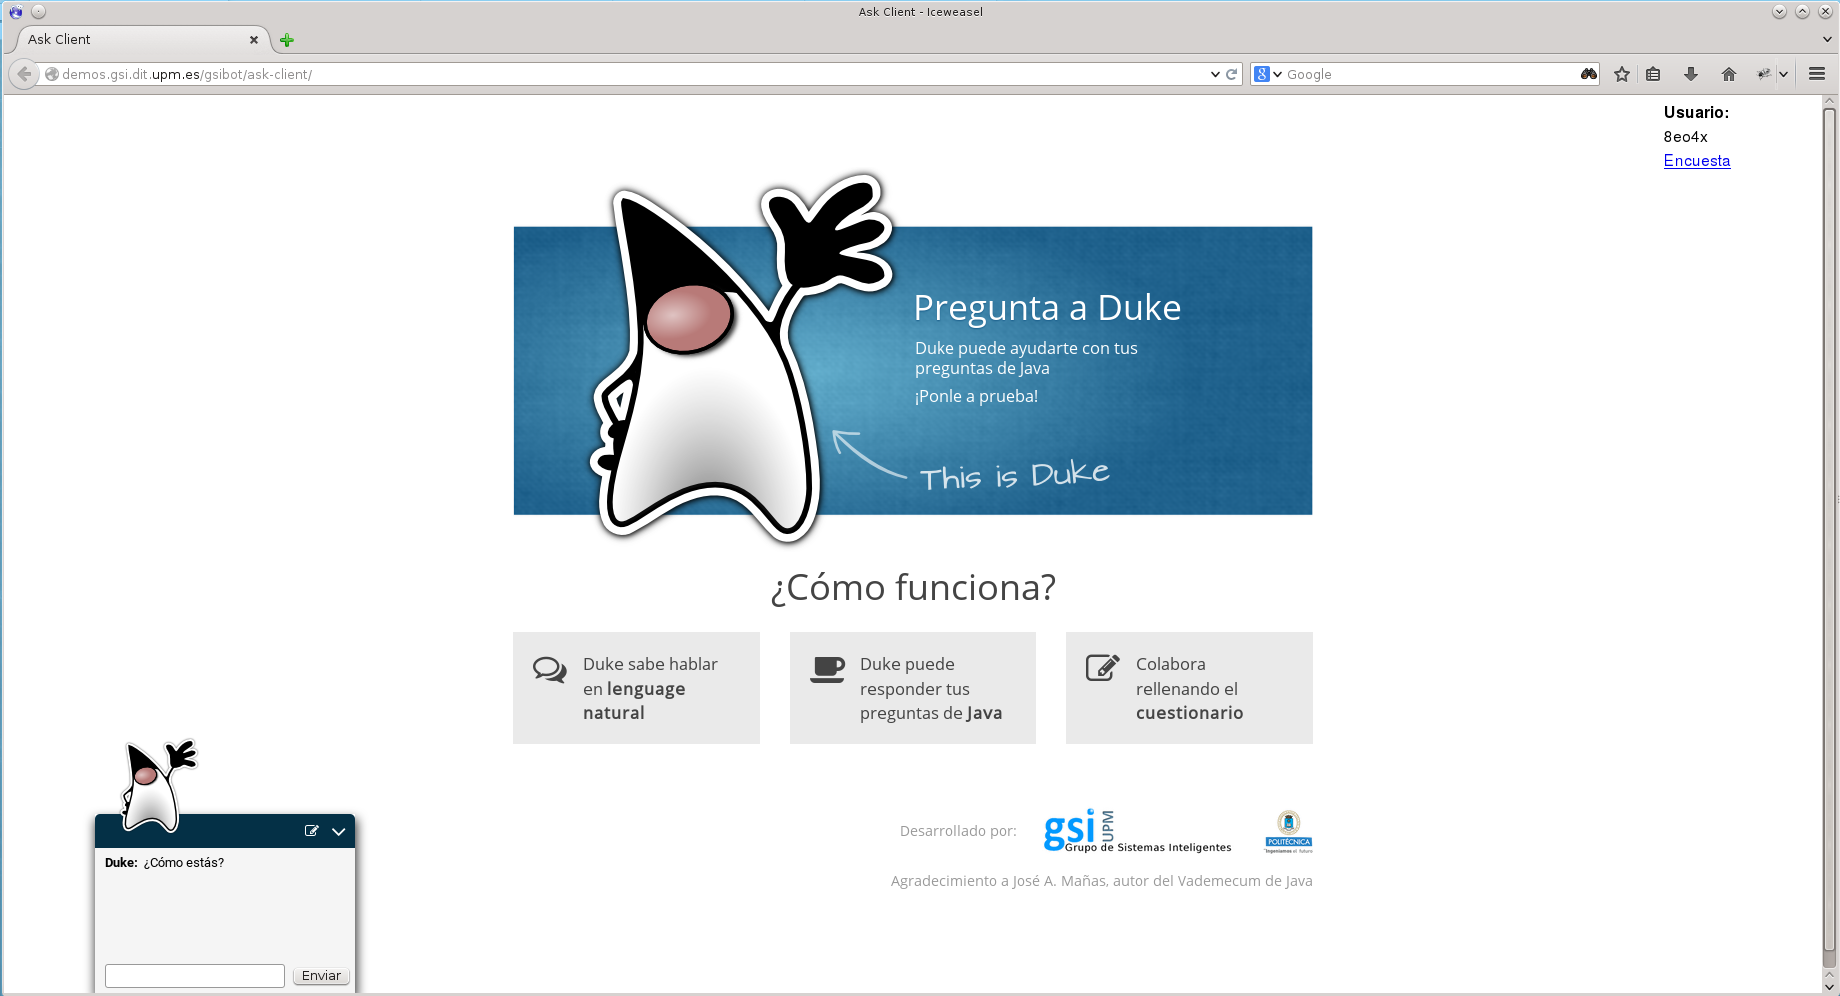
\includegraphics[width=0.7\textwidth]{img/screens/ask-client.png}
    \caption{Web interface for the client.}
    \label{fig:chat1}
\end{figure}


\section{Controller}
\label{sec:controllergsi}

The controller handles the requests received from the client described in the previous section, interacting with the required modules as needed, and interpreting the \ac{OoB} commands generated by each module. This module is very similar to the one described in section \ref{sec:frontendcon} of the previous chapter, and is developed using the same technologies. It follows the same functional model described in section \ref{subsec:functmodel}.

\subsection{Structural Model}

In this section we will describe the structure followed by the controller of this prototype. The relevant methods of said structure are shown in figure \ref{fig:gsi-methods1}.

\begin{figure}[!htbp]
    \centering
    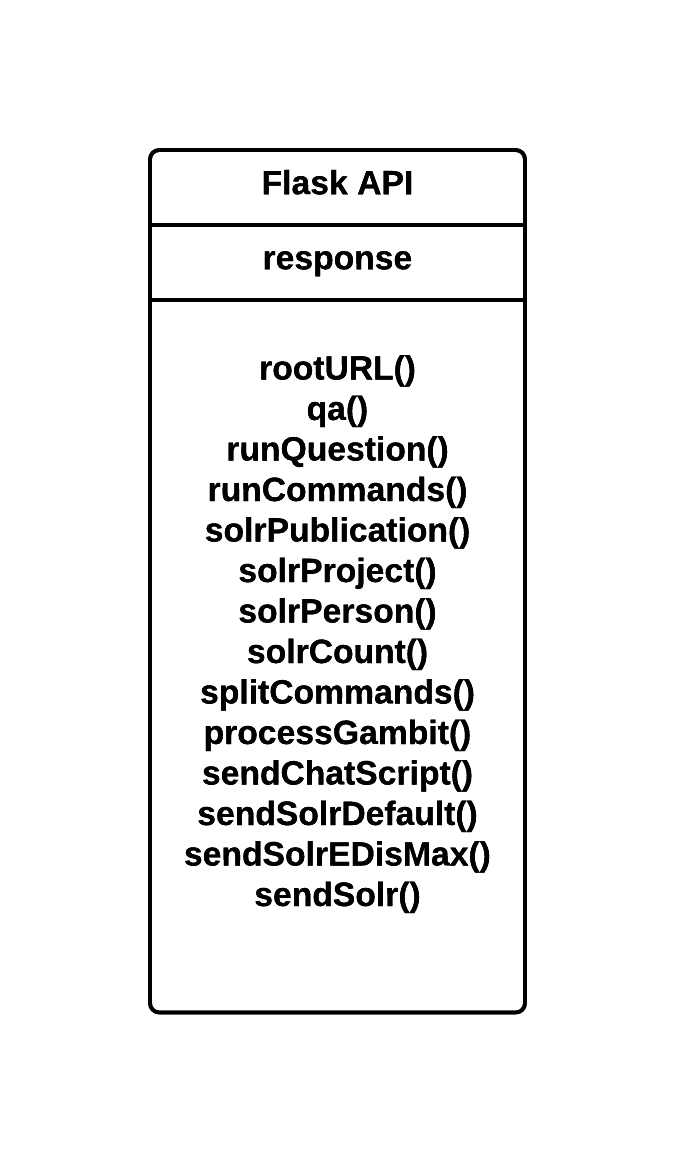
\includegraphics[width=0.4\textwidth]{img/prot2/controllerStructure.png}
    \caption{Front end controller structure}
    \label{fig:gsi-methods1}
\end{figure}

The function for each of those methods is described next:

\begin{itemize}
  \item \textbf{rootURL()} triggered when the base URL for the controller is requested, it acts in the same way as the qa() method.
  \item \textbf{qa()} Parsing the request parameters shown in table \ref{tab:fe-qparams}, this method will start the process to process the user question, and return the response once said process is complete, following the structure on table on table \ref{tab:fe-rparams}. 
  \item \textbf{runQuestion()} Send the question to ChatScript once, to generate the first \ac{OoB} commands and start processing them.
  \item \textbf{runCommands()} Parse the response from ChatScript and split the \ac{OoB} commands, in order to start processing each one of them, as well as their responses, adding commands to the queue as needed.
  \item \textbf{solrPublication()} When the user is asking about a publication, parse the parameters and perform the relevant Solr lookup.
  \item \textbf{solrProject()} Parse handle the queries to Solr when the question involves projects.
  \item \textbf{solrPerson()} Handle requests regarding members of the GSI.
  \item \textbf{solrCount()} When the user ask about quantities rather than about the documents themselves, perform the appropiate Solr lookup.
  \item \textbf{processGambit()} As a last resource, perform a broad search in Solr with the user query. This is further explained in section \ref{sec:solr}.
  \item \textbf{sendChatScript()} This function will process the interaction with ChatScript, both sending the questions and handling the responses. For more details, see section \ref{sec:chatbot}.
  \item \textbf{sendSolrDefault()} Given a question and no other parameters or information, this function will send said question to Solr, so it will go through the default processing. This is mainly unused.
  \item \textbf{sendSolrEDisMax()} Send the question to Solr using an \ac{eDisMax} query, usually for a gambit. 
  \item \textbf{sendSolr()} Send a direct query to solr. Mainly used by the rest of the solr lookup methods.
\end{itemize}

Finally, we will describe the \ac{OoB} commands that the system will be able to process.

\begin{itemize}
 \item \textbf{¬solrPublication} and \textbf{¬solrResponsePublication} this commands handle the interactions when the user question is about the publications.
 \item \textbf{¬solrProject} and \textbf{¬solrResponseProjects} are issued for the query and response when performing lookups about the projects.
 \item \textbf{¬solrPerson} and \textbf{¬solrResponsePerson} handle the queries for the lookups related with the GSI members.
 \item \textbf{¬solrCount} and \textbf{¬solrcounted} perform the query for the number of documents relevant to a given filter.
 \item \textbf{¬solrLinks} a special Solr search, looking for related topics in Solr. 
 \item \textbf{¬gambit} performs an \ac{eDisMax} search in Solr, with the user query.
 \item \textbf{¬gambitResponse} returns the response of the gambit \ac{eDisMax} query.
 \item \textbf{¬gambitUnknown} issued when the gambit does not return any relevant document.
 \item \textbf{¬resource} sets the URL to be shown to the user in the client.
\end{itemize}

The syntaxes of the commands is specified in table \ref{tab:gsi-commands}. \emph{\textcolor{red}{Update this table}}
\begin{center}
  \centering
  \begin{table}
    \begin{tabular*}{0.7\textwidth}{@{\extracolsep{\fill}} | c | c | p{0.35\textwidth} |}
      \hhline{|-|-|-|}
      \textbf{Command} & \textbf{Syntaxes} & \textbf{Description} \\ \hhline{|=|=|=|}
      ¬sendSolr & ¬sendSolr \textit{reqfield} \textit{doctitle} & Searchs in solr for the \textit{doctitle} and returns the \textit{reqfield} field.  \\ \hhline{|-|-|-|}
      \multirow{2}{*}{¬solrResponse} & ¬solrResponse \textit{unknown} & The requested document was not found in Solr. \\ \cline{2-3}
				     & ¬solrResponse \textit{reqfield} \textit{response} & Returns as \textit{response} the data of the field \textit{reqfield}. \\ \hhline{|-|-|-|}
      ¬solrLinks & ¬solrLinks \textit{linklist} & Asks for a search in Solr for the name of the topics given as an uri in the linklist \\ \hhline{|-|-|-|}
      ¬solrLinksResponse & ¬solrLinksResponse \textit{nameslist} & Sets the response for the ¬solrLinks command, returning the first name of the links. \\ \hhline{|-|-|-|}
      ¬gambit & ¬gambit \textit{topic}& Asks for a \ac{eDisMax} search on Solr, passing the full question. \\ \hhline{|-|-|-|}
      ¬gambitResponse & ¬gambitResponse \textit{gambittopic} & After performing an \ac{eDisMax} search, returns \textit{gambittopic} as the suggested topic. \\ \hhline{|-|-|-|}
      ¬gambitUnknown & ¬gambitUnknown & After performing an \ac{eDisMax} search, indicates that no relevant document has been found. \\ \hhline{|-|-|-|}
      ¬resource & ¬resource \textit{URL} & Sets \textit{URL} as the resource to be displayed in the client \\ \hhline{|-|-|-|}
      ¬label & ¬label \textit{topic} & Sets \textit{topic} as the concept of the response \\ \hhline{|-|-|-|}
      \end{tabular*}
    \caption{Parameters in the query sent back to the client.}
    \label{tab:gsi-commands}
  \end{table}
\end{center}


\section{Chatbot}
\label{sec:chatbotgsi}

Using the ChatScript chat engine, the Chatbot handles the conversation and process the natural language interactions with the user. However, to adapt to the fact that the documents stored in Solr for this prototype are not homogeneous, the rule structure has been changed.

\subsection{The rules}

We have separated the rules regarding different types of documents in one topic file per type, and therefore, we will have the following files and topics:

We have separated our topics across several files, each containing related topics, as well as the control script for the bot. We will start describing the control process, shown in listing~\ref{listing:cs-control}


\begin{itemize}
 \item \textbf{people.top} This file has the interactions regarding the members of the group, in the PEOPLE topic.
 \item \textbf{projects.top} with the topics regarding the projects.
 \item \textbf{publications.top} contains the topics relevant to the publications.
 \item \textbf{introductions.top} contains simple chat about the bot, as well as greetings and farewells.
 \item \textbf{mixed.top} in this file are stored topics with questions regarding more than one of the fields.
\end{itemize}

Finally, the control script used for this bot is very similar to the one provided by default with ChatScript, since we do not have the limitations regarding changing the language in this bot.

\emph{\textcolor{red}{Explain the control script?}}

\subsection{The server}

ChatScript provides two ways of interaction. For debugging purposes, it has a command line interface, and can also be deployed as a service listening in a TCP socket for user input. This server is what we have choose to use to interact with ChatScript. The full deployment instructions can be found in the appendix, and we will proceed to describe here the communication process.

As stated ChatScript listens on a TCP socket, waiting for requests containing three null separated strings, described in table~\ref{tab:cs-reqparamsgsi}

\begin{center}
  \centering
  \begin{table}
  \begin{center}
    \begin{tabular*}{0.6\textwidth}{@{\extracolsep{\fill}} | c | p{0.5\textwidth} |}
      \hhline{|-|-|}
      \textbf{Field} & \textbf{Description} \\ \hhline{|=|=|}
      user & The string identifying the user performing the question.  \\ \hhline{|-|-|}
      bot & The bot that the question is directed to, in case there are several bot available in the server. \\ \hhline{|-|-|}
      question & The user question \\ \hhline{|-|-|}
      \end{tabular*}
    \caption{Fields for the request to ChatScript}
    \label{tab:cs-reqparamsgsi}
    \end{center}
  \end{table}
\end{center}

The server will then return in the same connection the response generated using the process previously explained, and close the connection. If a new interaction is needed, a new socket will be opened, following the same process.
% \subsubsection{Using Spanish dictionaries}

%\emph{\textcolor{red}{It doesn't look viable to have spanish dicts in a timely manner.}}

\section{Solr instance}

In this section we will describe how the Solr instance has been configured for this system, as well as the search procedure. As in section \ref{sec:solr}, we are using Apache Solr 4.10.2, which will receive the queries from the controller described in section \ref{sec:controllergsi}. The Solr instance will contain a core with the data scrapped from the web page, allowing us to have all the date in a single place. %rephrase this?

\subsection{Solr Schema}

For this system, we have stored all the scrapped data in the same Solr core. Therefore, we can classify the fields according to the type of document they are associated with. Therefore, we will look at the fields grouping them according to said type of document:

\begin{itemize}
 \item \textbf{Stock solr fields:} Fields internal for Solr, we will not describe them here.
 \item \textbf{Document fields:} the fields scrapped from the web.
    \subitem \emph{Fields for the projects:} These fields are derived from the project exported structure.
    \subitem \emph{Fields for the members of the GSI}: Describing the people at the GSI, this fields are based on \ac{FOAF} fields.
    \subitem \emph{Fields for the publications:} Based on the bibtex ontology described in section \ref{subsec:bibtexrdf}.
 \item \textbf{searchField field:} this fields is generated concatenating fields from all three types of fields, to allow a default search with a single field.
\end{itemize}

A short description of each field, as well as the field types is shown in table \ref{tab:schema-gsifields}

\emph{\textcolor{red}{Fill this table. Maybe move it to an appendix?}}
\begin{center}
  \centering
  \begin{table}
  \begin{center}
    \begin{tabular*}{0.8\textwidth}{@{\extracolsep{\fill}} | c | c | c | p{0.3\textwidth} |}
      \hhline{|-|-|-|-|}
      \textbf{Field} & \textbf{Field Type} & \textbf{Type of document} & \textbf{Description} \\ \hhline{|=|=|=|=|}
      about & string & all & The object this document is describing. \\ \hhline{|-|-|-|-|}
      type & string & all & The object class for this document. \\ \hhline{|-|-|-|-|}
      journal & lowercase & Publication & The Journal associated with the publication. \\ \hhline{|-|-|-|-|}
      volume & string & Publication & The volume number \\ \hhline{|-|-|-|-|}
      year & string & Publication & The year for the publication \\ \hhline{|-|-|-|-|}
      month & lowercase & Publication & The month for the publication \\ \hhline{|-|-|-|-|}
      booktitle & text\_search & Publication & The title of the book the publication is associated with. \\ \hhline{|-|-|-|-|}
      --- & --- & --- & -- \\ \hhline{|-|-|-|-|}
      \end{tabular*}
    \caption{Fields in the Solr schema for the gsidata core.}
    \label{tab:schema-gsifields}
    \end{center}
  \end{table}
\end{center}

The ``text\_search'' field is based on the default English fields, and is defined as shown in listing \ref{listing:schemagsisearch}

\begin{center}
  \lstinputlisting[language=XML, captionpos=b, caption=Definition for the text\_search fieldType, label=listing:schemagsisearch, firstline=580, lastline=599]{code/prot2/schema.xml}
\end{center}

With this configuration we will perform the queries described in the next sections.

\subsection{Solr queries}

For this system, we have considered several types of queries. We have considered questions about the different objects and its relations, questions about quantifying specific subsets, and gambit queries. 

\subsubsection{Questions about quantities}

This query is perform when ChatScript identifies a question about the about of some type of document. This query will recover the number of documents in Solr matching the required criteria, and return it in an \ac{OoB} command. For example, for a question about the number of publications in 2014, the query will be as shown in listing \ref{listing:solrgsi1}. The meaning of each field is described next:

\begin{center} 
  \begin{lstlisting}[language=json, caption=Example json query for Solr, label=listing:solrgsi1]
   {
     "q" : "type:*bibtex* AND year:2014",
     "wt" : "json",
     "rows" : "0"
   }  
  \end{lstlisting}
\end{center}

\begin{itemize}
  \item \textbf{q} contains the actual query sent to the server, specifying the fields we are filtering with. In the example, we are searching for documents for year 2014. Since ``year'' is a field unique to publications, there is no real need to add the type filter.
  \item \textbf{wt} the format the data will be returned in. In the example, we want the data in json format.
  \item \textbf{rows} the number of documents to return. Since we only want the actual result count, rather than the documents, in the example it is set to 0
\end{itemize}

This search will return a json with the number of documents matching the criteria, which in turn will be pass to ChatScript, generating the appropriate \ac{NL} response.

\subsubsection{General questions}

ChatScript can also identify general questions about the different objects stored in Solr. In those cases, Solr will perform a regular search, returning the document with the highest score, which will them offered to the user as a response.

\emph{\textcolor{red}{Add example query for this}}

\subsubsection{Gambit queries}

In the event that ChatScript is incapable of identify the question the user is making, the system will perform an \ac{eDisMax} query, looking for a match in the relevant fields for each document type, and offering the answer only if the score of the match is over a predetermined minimum score.